\documentclass[10pt]{beamer}

\usetheme{bjeldbak}
\setbeamertemplate{headline}{}
%\usetheme[titleformat=smallcaps]{metropolis}
\usepackage{appendixnumberbeamer}

%\usepackage{booktabs}
%\usepackage[scale=2]{ccicons}
\usepackage{tcolorbox}

%\usepackage{floatrow}

%\usepackage{minted}
%\usemintedstyle{trac}

% For the 68 colors
\usepackage{xcolor}
\definecolor{ao}{rgb}{0.0, 0.5, 0.0}

\usepackage{pgfplots}
\usepgfplotslibrary{dateplot}

\usepackage{xspace}
\newcommand{\themename}{\textbf{\textsc{metropolis}}\xspace}


\usepackage{subfig}
\usepackage[absolute,overlay]{textpos}
\usepackage{tikz}



\usepackage{times}
\usepackage{amsmath}
\usepackage{verbatim}
\usetikzlibrary{arrows,shapes}


\usepackage{mathtools}

\newcommand{\verteq}{\rotatebox{90}{$\,=$}}
\newcommand{\equalto}[2]{\underset{\scriptstyle\overset{\mkern4mu\huge \verteq}{#2}}{#1}}


\newcommand{\bra}[1]{\left\langle #1\right|}
\newcommand{\ket}[1]{\left| #1\right\rangle}
\newcommand{\braket}[2]{\langle #1 \mid #2 \rangle}
\newcommand{\avg}[1]{\left< #1 \right>}
\newcommand{\ii}{\mathrm{i}}
\DeclareMathOperator{\sech}{sech}



%%%%%%%%%%%%%%%%%%%%%%%%%
%%%%% For Timeline %%%%%%

% http://tex.stackexchange.com/questions/196794/how-can-you-create-a-vertical-timeline

%\usepackage[T1]{fontenc}
\usepackage[utf8]{inputenc}
\usepackage{charter}
\usepackage{environ}
\usepackage{tikz}
\usetikzlibrary{calc,matrix}

\makeatletter
\let\matamp=&
\catcode`\&=13
\makeatletter
\def&{\iftikz@is@matrix
  \pgfmatrixnextcell
  \else
  \matamp
  \fi}
\makeatother

\newcounter{lines}
\def\endlr{\stepcounter{lines}\\}

\newcounter{vtml}
\setcounter{vtml}{0}

\newif\ifvtimelinetitle
\newif\ifvtimebottomline
\tikzset{description/.style={
  column 2/.append style={#1}
 },
 timeline color/.store in=\vtmlcolor,
 timeline color=red!80!black,
 timeline color st/.style={fill=\vtmlcolor,draw=\vtmlcolor},
 use timeline header/.is if=vtimelinetitle,
 use timeline header=false,
 add bottom line/.is if=vtimebottomline,
 add bottom line=false,
 timeline title/.store in=\vtimelinetitle,
 timeline title={},
 line offset/.store in=\lineoffset,
 line offset=4pt,
}

\NewEnviron{vtimeline}[1][]{%
\setcounter{lines}{1}%
\stepcounter{vtml}%
\begin{tikzpicture}[column 1/.style={anchor=east},
 column 2/.style={anchor=west},
 text depth=0pt,text height=1ex,
 row sep=1ex,
 column sep=1em,
 #1
]
\matrix(vtimeline\thevtml)[matrix of nodes]{\BODY};
\pgfmathtruncatemacro\endmtx{\thelines-1}
\path[timeline color st] 
($(vtimeline\thevtml-1-1.north east)!0.5!(vtimeline\thevtml-1-2.north west)$)--
($(vtimeline\thevtml-\endmtx-1.south east)!0.5!(vtimeline\thevtml-\endmtx-2.south west)$);
\foreach \x in {1,...,\endmtx}{
 \node[circle,timeline color st, inner sep=0.15pt, draw=white, thick] 
 (vtimeline\thevtml-c-\x) at 
 ($(vtimeline\thevtml-\x-1.east)!0.5!(vtimeline\thevtml-\x-2.west)$){};
 \draw[timeline color st](vtimeline\thevtml-c-\x.west)--++(-3pt,0);
 }
 \ifvtimelinetitle%
  \draw[timeline color st]([yshift=\lineoffset]vtimeline\thevtml.north west)--
  ([yshift=\lineoffset]vtimeline\thevtml.north east);
  \node[anchor=west,yshift=16pt,font=\large]
   at (vtimeline\thevtml-1-1.north west) 
   {%\textsc{Timeline \thevtml}: 
   \textit{\vtimelinetitle}};
 \else%
  \relax%
 \fi%
 \ifvtimebottomline%
   \draw[timeline color st]([yshift=-\lineoffset]vtimeline\thevtml.south west)--
  ([yshift=-\lineoffset]vtimeline\thevtml.south east);
 \else%
   \relax%
 \fi%
\end{tikzpicture}
}


%%%% Timeline END %%%%%%%
%%%%%%%%%%%%%%%%%%%%%%%%%


\title{Neutrino Oscillations in Matter}
\subtitle{PhD Candidacy Exam}
\date{April 19, 2016}
\author{Lei Ma\\
{\bf{Supervisor}}: Huaiyu Duan}
\institute{Department of Physics\\
UNM}
% \titlegraphic{\hfill
\includegraphics[height=1.5cm]{logo.pdf}}

\begin{document}

  {%
    \setbeamertemplate{headline}{}
    \frame{\titlepage}
  }

%\maketitle % The reason why two title pages

\begin{frame}{Outline}
  \setbeamertemplate{section in toc}[sections numbered]
  \tableofcontents
\end{frame}

\section{Introduction}


\subsection{History of Neutrinos}

\begin{frame}[fragile]{Neutrino Timeline}


\begin{vtimeline}[description={text width=\textwidth}, 
 row sep=2ex, 
 use timeline header,
 timeline title={History of Neutrino (Partial)}]
1930 & Pauli, letter to "Radioactive Ladies and Gentlemen"\endlr
1933 & Fermi, the name "neutrino" \endlr
1956 & Reines \& Cowan, first neutrino evidence \endlr
1957 & \textbf{Pontecorvo, theory of neutrino oscillations} \endlr
1968 & Homestake, first solar neutrino detection \endlr
%1969 & Gribov \& Pontecorvo, solar neutrino oscillations \endlr
1978 \& 1985 & \textbf{Wolfenstein \& Mikheyev \& Smirnov, MSW effect} \endlr
1987 & Kamioka mine \& Morton salt mine, SN1987A neutrino\endlr
1998 \& 2001 & Super-Kamiokande \& SNO, solar neutrino oscillations \endlr
\end{vtimeline}


\end{frame}







%%%% Neutrino as a Particle
\subsection{What are Neutrinos}

\begin{frame}{What are Neutrinos?}

\begin{figure}
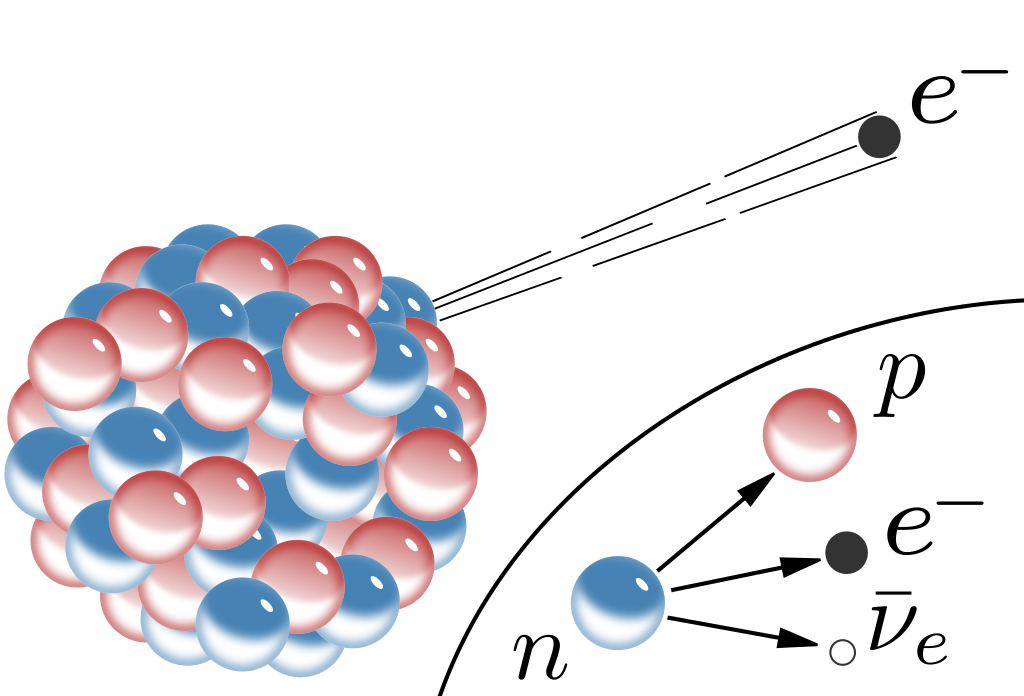
\includegraphics[width=0.9\linewidth,height=0.9\textheight,keepaspectratio]{assets/beta-decay.png}
\caption*{Beta decay and antineutrino production. Source: Beta\_Decay@Wikipedia}
\end{figure}


\end{frame}




\begin{frame}{What are Neutrinos?}

\begin{minipage}[\textheight]{\textwidth}
\begin{columns}[T]

\begin{column}{0.6\textwidth}
\begin{figure}
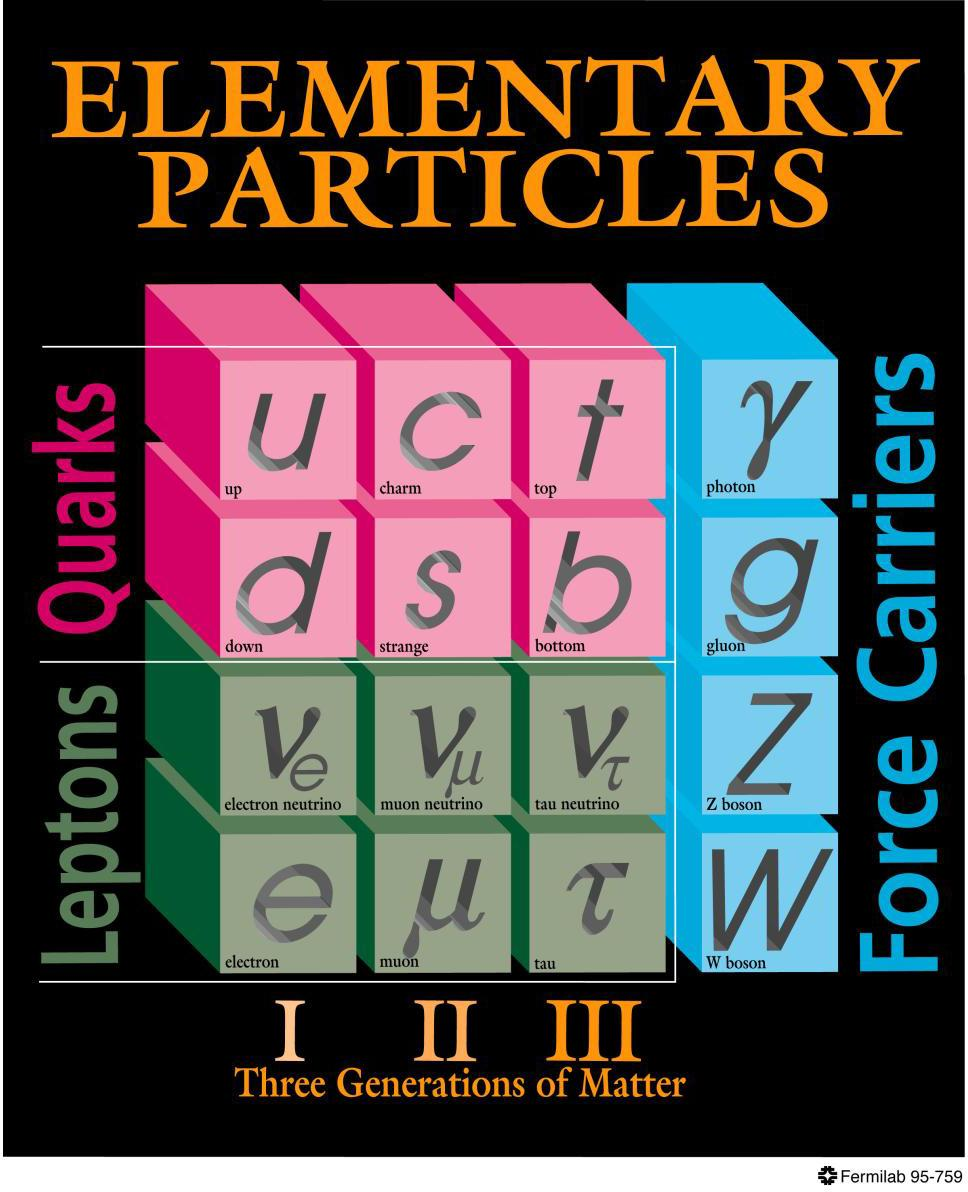
\includegraphics[width=0.9\linewidth,height=0.8\textheight,keepaspectratio]{assets/elementary-particles.jpg}
\caption*{Table of elementary particles. Source: Fermilab} % http://www-d0.fnal.gov/Run2Physics/WWW/results/final/TOP/T06C/T06C.html
\end{figure}
\end{column}

\begin{column}{0.4\textwidth}


    \begin{itemize}
    \item[] Neutrinos are
    \item Fermions,
    \item electrically neutral,
    \item \textbf{light}.
    \end{itemize}



\only<1-1>{
\begin{figure}
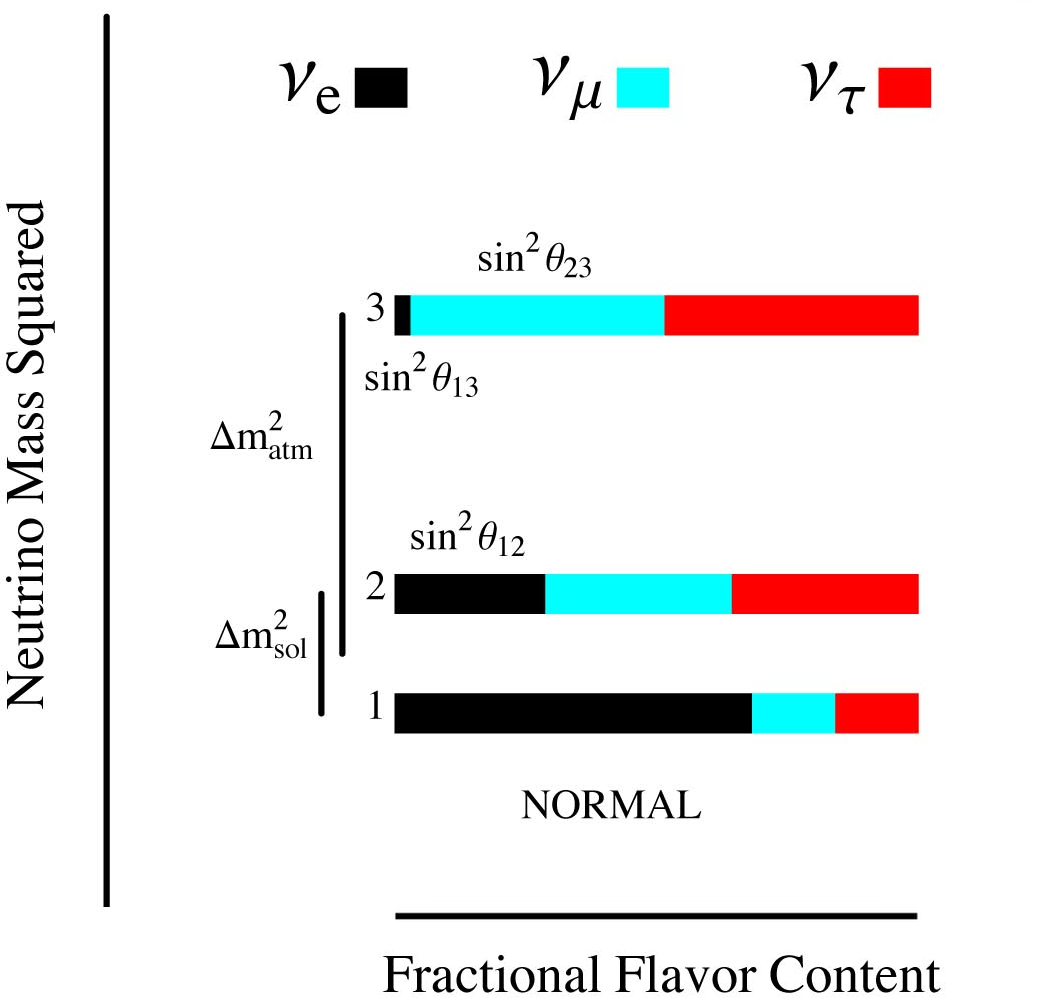
\includegraphics[width=\textwidth]{assets/neutrino-normal-hierarchy.png}
\caption*{Adapted from Olga Mena \& Stephen Parke, 2004}
\end{figure}
}

\only<2-2>{
\begin{figure}
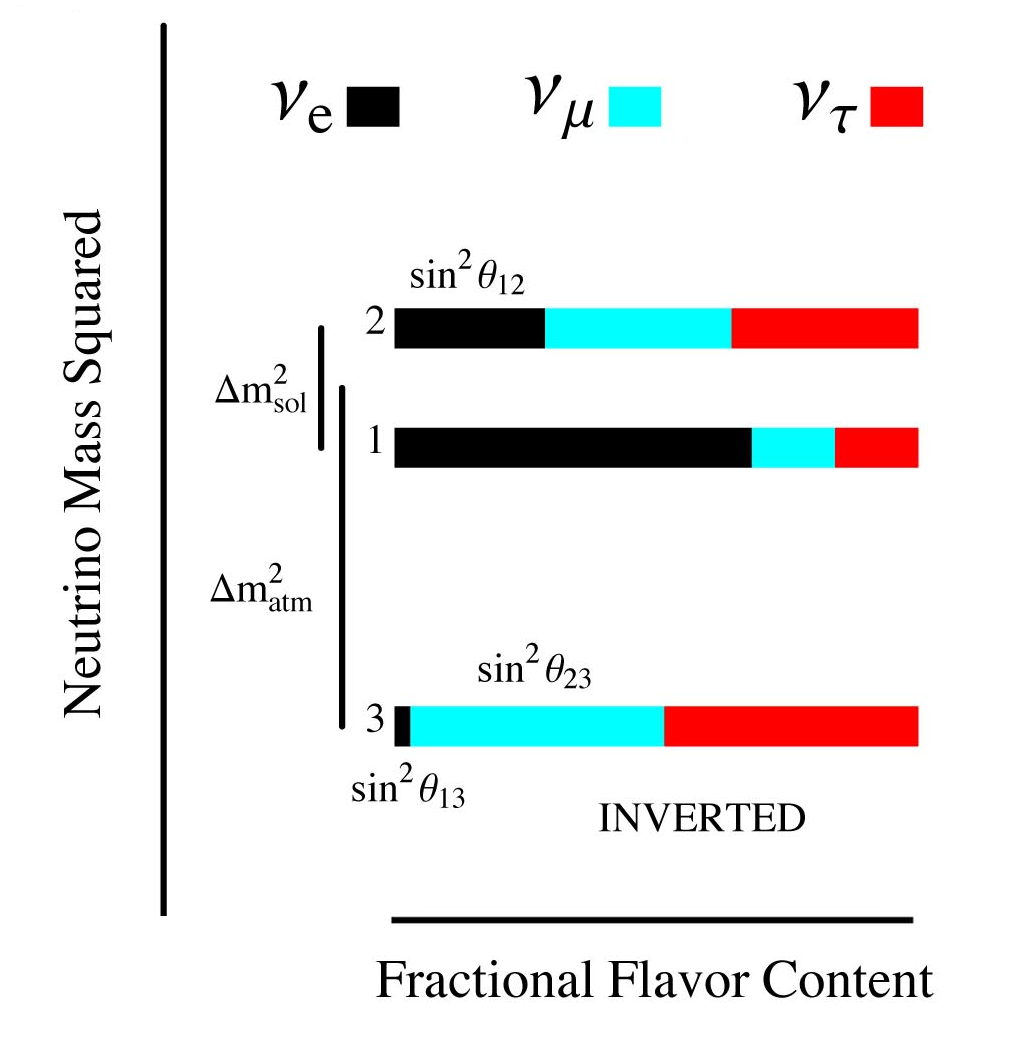
\includegraphics[width=\textwidth]{assets/neutrino-inverted-hierarchy.png}
\caption*{Adapted from Olga Mena \& Stephen Parke, 2004}
\end{figure}
}

\end{column}


\end{columns}
\end{minipage}

\end{frame}



%%%%% Neutrino Oscillations %%%%%%%%%

\subsection{Neutrino Oscillations}





\begin{frame}{What is Neutrino Oscillation?}

\setbeamercovered{invisible}


\only<1-1>{

\begin{tcolorbox}
\begin{equation*}
  \equalto{\textbf{\large Neutrino Oscillation} }{ \textbf{\large Neutrino Flavor Conversion } }
\end{equation*}

\end{tcolorbox}


\begin{figure}
    \centering
    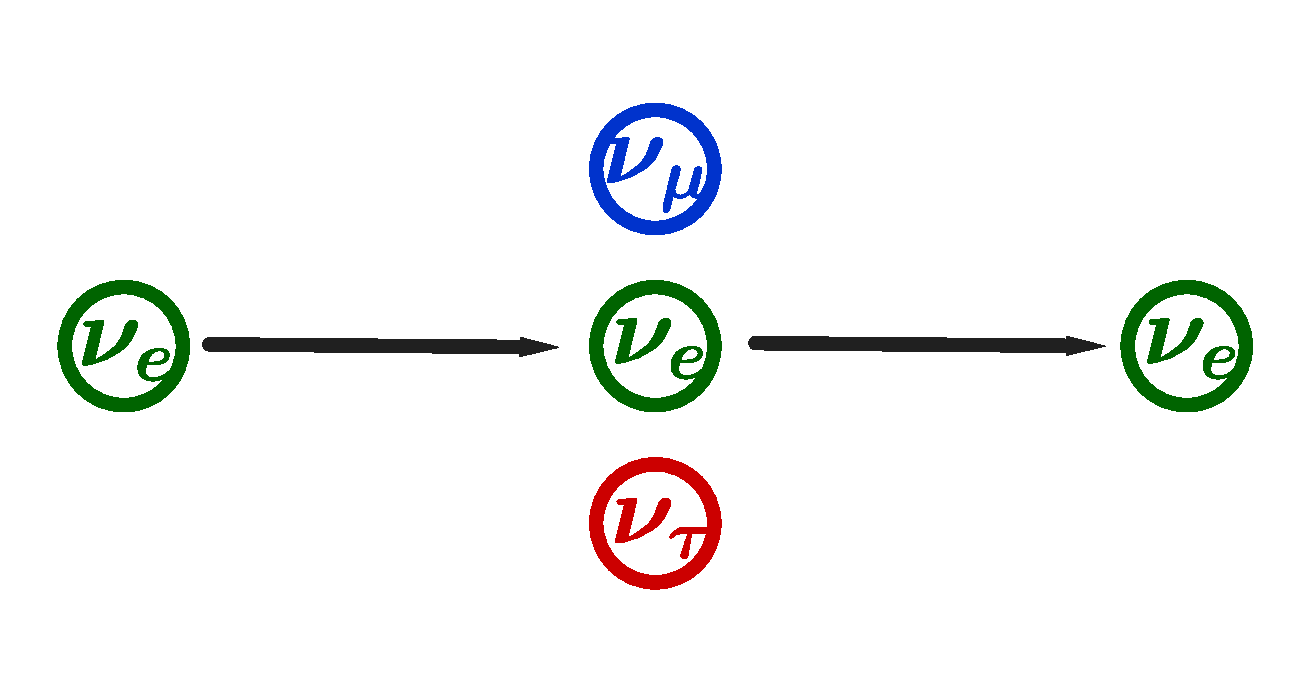
\includegraphics[width=\textwidth]{assets/neutrino-oscillations-illustration.eps}
    \caption*{Neutrino Oscillation}
\end{figure}

}


\only<2-2>{

\begin{figure}
    \centering
    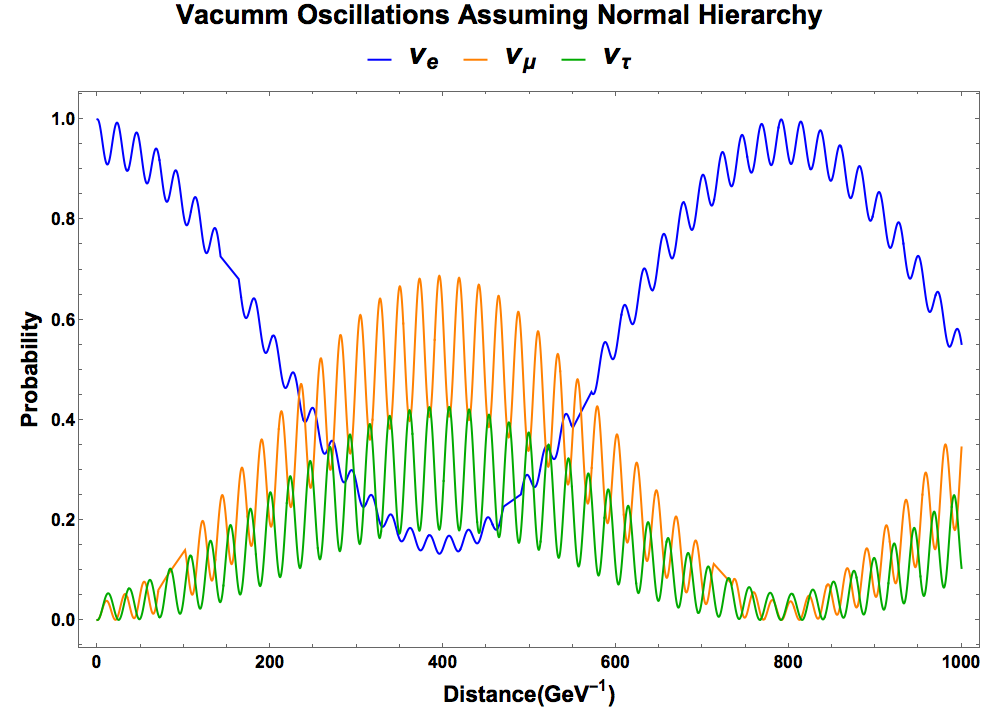
\includegraphics[width=0.9\textwidth]{assets/vacuum-oscillations-3-flavor.png}
    \caption*{Survival probability}
\end{figure}

}




\end{frame}


\subsection{Solar Neutrino Problem}

\begin{frame}{Solar Neutrinos}

\begin{tcolorbox}[title=Solar Neutrinos]
{\color{gray}pp chain}, $\mathrm{{}^7Be}$, $\mathrm{{}^8B}$, pep, CNO
\end{tcolorbox}

\begin{figure}
    \centering
    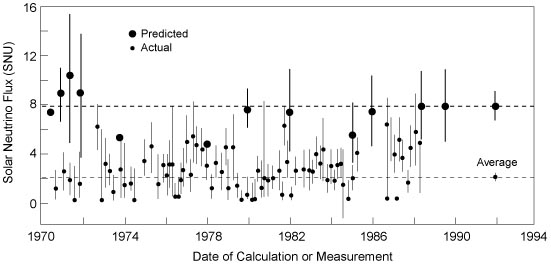
\includegraphics[width=0.8\textwidth]{assets/chlorine-detector-solar-neutrinos.jpg} %https://ase.tufts.edu/cosmos/print_images.asp?id=37
    \caption*{Chlorine detector (Homestake experiment) results and theory predictions. SNU: 1 event for $10^{36}$ target atoms per second.}
\end{figure}


% \begin{figure}
% \centering
% 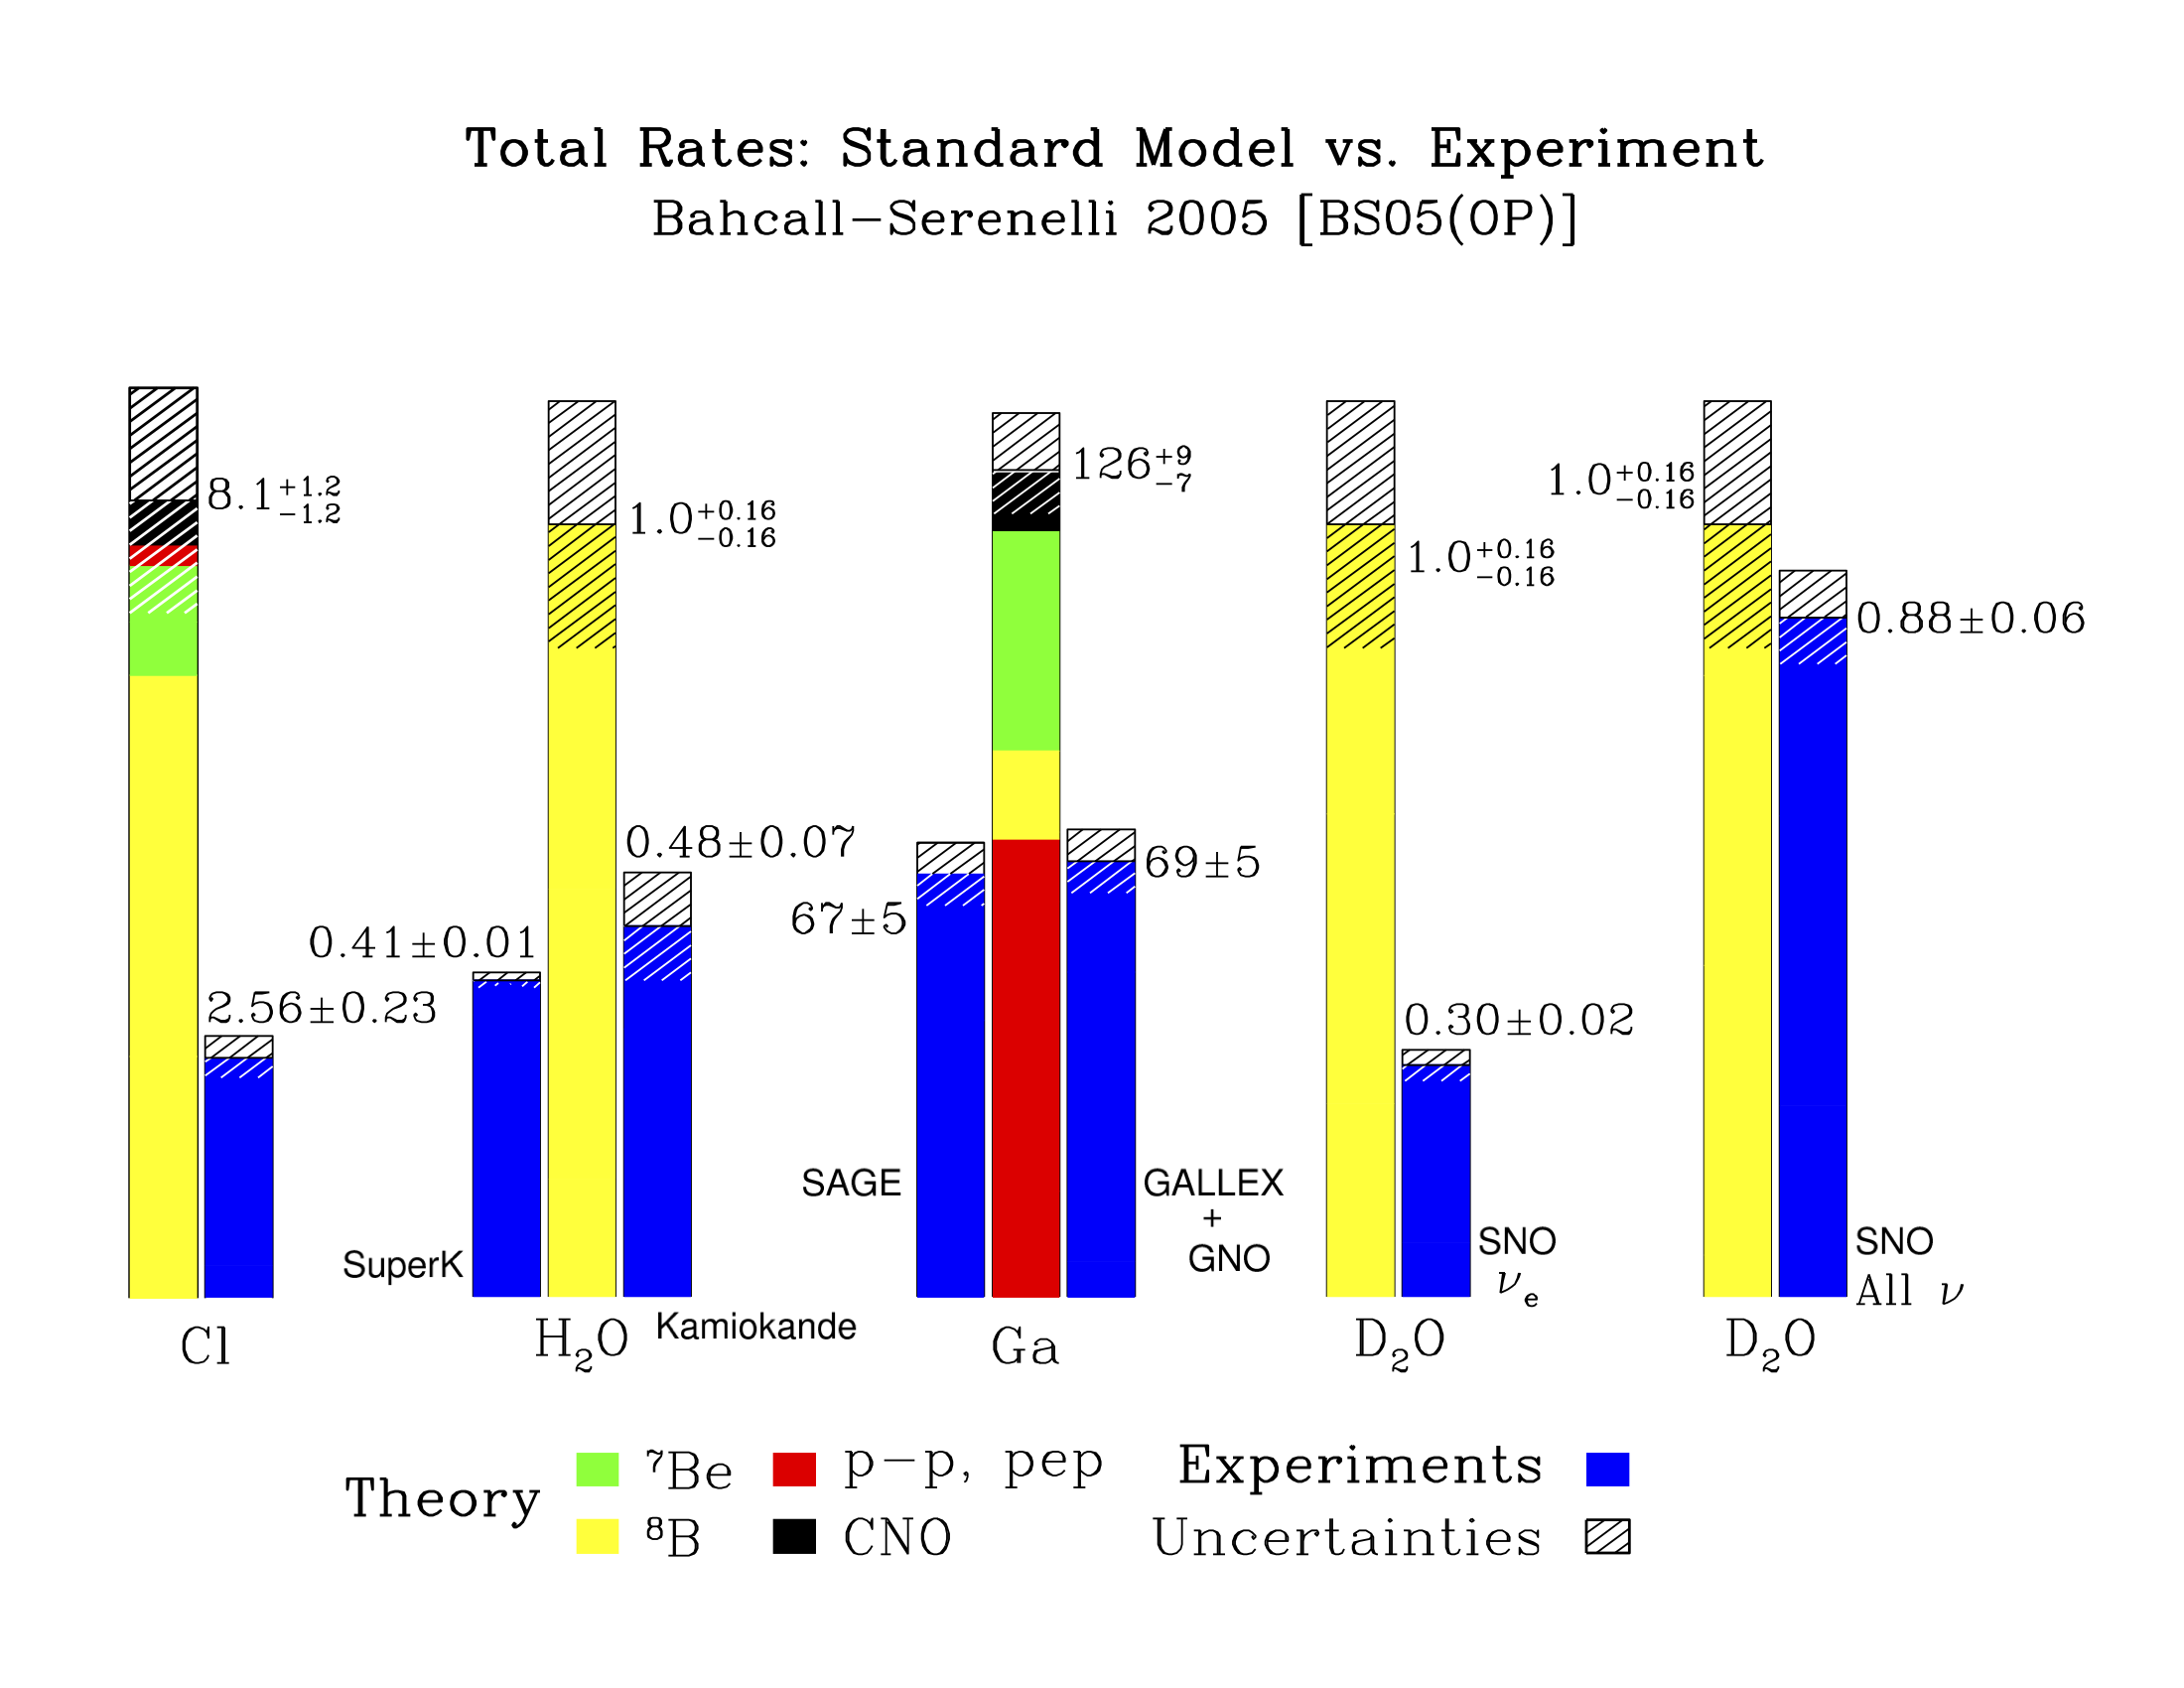
\includegraphics[width=0.8\textwidth]{assets/colortheoryvsexp.png}
% \caption*{Less electron flavor neutrinos observed in experiments than the Standard Solar Model prediction. Bahcall \& Serendelli, 2005}
% \end{figure}


    
\end{frame}




%%%%%% Why Neutrinos Oscillate? %%%%%%%%%

\subsection{Why Oscillations}

% For every picture that defines or uses external nodes, you'll have to
% apply the 'remember picture' style. To avoid some typing, we'll apply
% the style to all pictures.
\tikzstyle{every picture}+=[remember picture]

% By default all math in TikZ nodes are set in inline mode. Change this to
% displaystyle so that we don't get small fractions.
\everymath{\displaystyle}


\begin{frame}[fragile]{Why Do Neutrinos Oscillate?}

\begin{tcolorbox}[title=Equation of Motion]

\begin{equation*}
i\partial_x \Psi = \mathbf H \Psi
\end{equation*}

\end{tcolorbox}




\begin{itemize}
\item Basis: Hamiltonian diagonalized basis/mass eigenbasis/propagation eigenbasis, $\ket{\nu_1}$ and $\ket{\nu_2}$.

\item
\begin{equation*}
    \mathbf H = - \frac{\omega_v}{2}\boldsymbol{\sigma_3}, \qquad \text{where } \omega_v = \frac{\delta m^2}{2E}=\frac{m_2^2 - m_1^2}{2E} .
\end{equation*}



\item The system can be solved given initial condition of the wave function $(\braket{\nu_1}{\Psi(0)},\braket{\nu_2}{\Psi(0)} )^T$,
\begin{equation*}
    \begin{pmatrix}
    \braket{\nu_1}{\Psi(t)} \\
    \braket{\nu_2}{\Psi(t)}
    \end{pmatrix} = \begin{pmatrix}
    \braket{\nu_1}{\Psi(0)} \exp\left( \ii  \omega_v x /2 \right) \\
    \braket{\nu_2}{\Psi(0)} \exp\left( -\ii  \omega_v x/2 \right)
    \end{pmatrix} 
\end{equation*}


\end{itemize}




\end{frame}


%%%%%%%%%



\begin{frame}[fragile]{Why Do Neutrinos Oscillate?}


\begin{tcolorbox}[title=Flavor basis]


Neutrino wave function in flavor basis $(\psi_e, \psi_x)^T$ is related to state in energy eigenbasis $(\psi_1,\psi_2)^T$ through

\begin{equation*}
\begin{pmatrix}\psi_e \\ \psi_x\end{pmatrix} = \begin{pmatrix}  \cos\theta  & \sin\theta \\ -\sin\theta  & \cos\theta \end{pmatrix}   \begin{pmatrix}\psi_1 \\ \psi_2\end{pmatrix}
\end{equation*}


\end{tcolorbox}

\pause

\begin{tcolorbox}[title=Hamiltonian $\mathbf H$]

\begin{columns}[T] % align columns
\begin{column}{.49\textwidth}

\centering Energy eigenbasis


\begin{align*}
&\frac{\omega_v}{2}\begin{pmatrix}
-1  & 0 \\
0 & 1
\end{pmatrix}\\
=&
-\frac{\omega_v}{2}\boldsymbol{ \sigma_3 }
\end{align*}



\end{column}%
\hfill%

\begin{column}{.49\textwidth}

\centering Flavor eigenbasis

\begin{align*}
&\frac{\omega_v}{2}\begin{pmatrix} -\cos 2\theta_v & \sin 2 \theta_v \\ \sin 2\theta_v & \cos 2\theta_v  \end{pmatrix} \\
=&
\frac{\omega_v}{2}\left( - \cos 2\theta_v\boldsymbol{ \sigma_3 } + \sin 2\theta_v \boldsymbol{\sigma_1} \right)
\end{align*}

\end{column}%
\end{columns}

\end{tcolorbox}



\end{frame}





\begin{frame}[fragile]{Nature of Neutrino Oscillation}
\setbeamercovered{invisible}



\begin{tcolorbox}[title=Survival Probability]

\begin{equation*}
P(\ket{\nu_e}\to\ket{\nu_x})  =  \sin^2(2\theta_v) \frac{ 1- \cos \left( \omega_v x \right) }{2}
\end{equation*}
\alert{Mixing angle $\to$ Flavor oscillation amplitude\\
Eigenenergies $\to$ Oscillation frequency}


\end{tcolorbox}


\end{frame}




%%%%%%%%%%%%%%%%%%%%%%%%%%%%%%%%%%%%%%%%%%%%%%%%%%%%%%%%%%%%%%%%%%
%%%%%%%%%%%%%%%%%%%% Matter Effect %%%%%%%%%%%%%%%


\section{Matter Effect}


\subsection{Matter Interaction}


\begin{frame}{Matter Interaction}


\begin{tcolorbox}[title=PLACEHOLDER]
SHOULD ADD IN WHY MATTER INTERACTION IS LIKE THIS.
\end{tcolorbox}


\end{frame}





% For every picture that defines or uses external nodes, you'll have to
% apply the 'remember picture' style. To avoid some typing, we'll apply
% the style to all pictures.
\tikzstyle{every picture}+=[remember picture]


% By default all math in TikZ nodes are set in inline mode. Change this to
% displaystyle so that we don't get small fractions.
\everymath{\displaystyle}



\begin{frame}{Matter Interaction}
\tikzstyle{na} = [baseline=-.5ex]




\begin{itemize}
    \item[] Hamiltonian with Matter Interaction in Flavor Basis  ($\omega_v=\delta m^2/2E$):
        \tikz[na] \node[coordinate] (n1) {};
\end{itemize}


\only<1-1>{
\begin{equation*}
    \mathbf{H} = 
    \tikz[baseline]{
            \node[fill=blue!20,anchor=base] (t1)
            {$ \frac{\omega_v}{2}\begin{pmatrix} -\cos 2\theta_v & \sin 2 \theta_v \\ \sin 2\theta_v & \cos 2\theta_v  \end{pmatrix} $}
            } + 
            \tikz[baseline]{
            \node[fill=red!20, anchor=base] (t2)
            {$ 
            \sqrt{2}G_F n_e(x) \begin{pmatrix}
            1 & 0 \\
            0 & 0
            \end{pmatrix}
            $};
        }
\end{equation*}



}




\only<2-2>{
\begin{equation*}
    \mathbf{H} = 
    \tikz[baseline]{
            \node[fill=blue!20,anchor=base] (t1)
            {$ \frac{\omega_v}{2}\begin{pmatrix} -\cos 2\theta_v & \sin 2 \theta_v \\ \sin 2\theta_v & \cos 2\theta_v  \end{pmatrix} $}
            } + 
            \tikz[baseline]{
            \node[fill=red!20, anchor=base] (t2)
            {$ 
            \frac{\sqrt{2}G_F n_e(x)}{2} \begin{pmatrix}
            1 & 0 \\
            0 & -1
            \end{pmatrix}
            $};
        }
\end{equation*}

}

\only<3-3>{
\begin{equation*}
    \mathbf{H} = 
    \tikz[baseline]{
            \node[fill=blue!20,anchor=base] (t1)
            {$ \frac{\omega_v}{2}\left( - \cos 2\theta_v \boldsymbol{\sigma_3} + \sin 2\theta_v \boldsymbol{\sigma_1} \right) $}
            } + 
            \tikz[baseline]{
            \node[fill=red!20, anchor=base] (t2)
            {$ 
            \frac{\sqrt{2}G_F n_e(x)}{2} \boldsymbol{\sigma_3}
            $};
        }
\end{equation*}

}

\only<4->{
\begin{equation*}
    \mathbf{H} = 
    \tikz[baseline]{
            \node[fill=blue!20,anchor=base] (t1)
            {$ \frac{\omega_v}{2}\left( - \cos 2\theta_v \boldsymbol{\sigma_3} + \sin 2\theta_v \boldsymbol{\sigma_1} \right) $}
            } + 
            \tikz[baseline]{
            \node[fill=red!20, anchor=base] (t2)
            {$ 
            \frac{\lambda(x)}{2} \boldsymbol{\sigma_3}
            $};
        }
\end{equation*}

}


\begin{itemize}
    \item Vacuum Hamiltonian
        \tikz[na]\node [coordinate] (n2) {};
    \item Matter interaction
        \tikz[na]\node [coordinate] (n3) {};
    \item<4-> $\lambda(x) = \sqrt{2}G_F n_e(x)$ 
\end{itemize}





% Now it's time to draw some edges between the global nodes. Note that we
% have to apply the 'overlay' style.
\begin{tikzpicture}[overlay]
        \path[->]<1-> (n2) edge [bend right] (t1);
        \path[->]<1-> (n3) edge [bend right=20] (t2);
\end{tikzpicture}

\only<4->{
\begin{tcolorbox}[title=Hamiltonian with Matter Potential]

\begin{equation*}
    \mathbf{H} = \frac{\lambda(x) - \omega_v \cos 2\theta_v}{2} \boldsymbol{\sigma_3} + \frac{ \omega_v \sin 2\theta_v}{2} \boldsymbol{\sigma_1}
\end{equation*}

\end{tcolorbox}
}




\end{frame}





%%%%%%%%%%%%%%%%%
\subsection{MSW Effect}

\begin{frame}{MSW Effect}



\begin{tcolorbox}[title=Hamiltonian in Vacuum]

\begin{equation*}
    \mathbf{H} = \frac{\omega_v \cos 2\theta_v }{2} \boldsymbol{\sigma_3} + \frac{ \omega_v \sin 2\theta_v}{2} \boldsymbol{\sigma_1}
\end{equation*}

\end{tcolorbox}


\begin{tcolorbox}[title=Hamiltonian with Matter Potential]

\begin{equation*}
    \mathbf{H} = \frac{  {\color{red}\omega_m(x) }    {\color{blue}\cos 2\theta_m(x)}  }{2} \boldsymbol{\sigma_3} + \frac{ {\color{red}\omega_m(x) }   {\color{red}\sin 2\theta_m(x) } }{2} \boldsymbol{\sigma_1},
\end{equation*}

where

\begin{align*}
    {\color{red}\omega_m(x) } =& \omega_v\sqrt{ \left(\frac{\lambda}{\omega_v} - \cos 2\theta_v \right)^2 + \sin^2 2\theta_v  }  ,\\
    {\color{blue}\tan 2\theta_m(x)} = & \sin 2\theta_v /\left(\cos 2\theta_v - \frac{\lambda(x)}{\omega_v} \right).
\end{align*}

\end{tcolorbox}






\end{frame}





\begin{frame}{Constant Matter Density}

\begin{tcolorbox}[title=Transition Probability for Constant Matter Density]


\begin{equation*}
P(\ket{\nu_e}\to\ket{\nu_x})  = \frac{1}{2} {\color{blue}\sin^2(2\theta_m)} \left[ 1- \cos \left( {\color{red}\omega_m} x \right) \right]
\end{equation*}

\only<1-1>{
where
\begin{align*}
    {\color{red}\omega_m(x) } =& \omega_v\sqrt{ \left(\frac{\lambda}{\omega_v} - \cos 2\theta_v \right)^2 + \sin^2 2\theta_v  }  ,\\
    {\color{blue}\tan 2\theta_m(x)} = & \sin 2\theta_v /\left(\cos 2\theta_v - \frac{\lambda(x)}{\omega_v} \right)  .
\end{align*}
}

\end{tcolorbox}


% \only<2->{
% \begin{itemize}
%     \item Oscillation amplitude depends on $\theta_m$
%     \item Oscillation angular frequency is
% \begin{equation*}
%     \omega_m \geq \omega_v \sin 2\theta_v
% \end{equation*}

% \end{itemize}
% }


\end{frame}




%%%%%%% MSW Effect %%%%%%%%%

\begin{frame}{MSW Effect}

\setbeamercovered{invisible}



\begin{equation*}
    \mathbf{H} = \frac{\lambda(x) - \omega_v \cos 2\theta_v}{2} \boldsymbol{\sigma_3} + \frac{ \omega_v \sin 2\theta_v}{2} \boldsymbol{\sigma_1}
\end{equation*}


\begin{equation*}
    \begin{pmatrix}
    \nu_{e}\\
    \nu_{x}
    \end{pmatrix} =  \begin{pmatrix}
    \cos \theta_m(x) & \sin \theta_m(x)\\
    -\sin \theta_m(x) & \cos \theta_m(x)
    \end{pmatrix}
    \begin{pmatrix}
    \nu_{1m}\\
    \nu_{2m}
    \end{pmatrix}
\end{equation*}








\begin{figure}
\centering
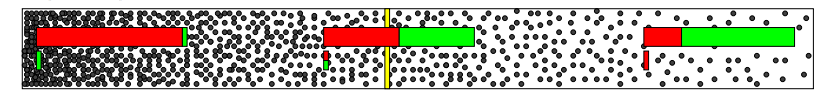
\includegraphics[width=0.9\textwidth]{assets/msw_and_density.png}
\caption*{Yellow bar is the resonance point. Smirnov, 2003.}
\label{fig:msw_and_density}
\end{figure}



\end{frame}





%%%%%%%%%%%%%%%%%%%%%%%%%%%%%%%%%%%%%%%%%%%%%%%%%%%%%%%%%%%%%%%%%%
%%%%%%%%%%%%%%%%%%%% Parametric Effect %%%%%%%%%%%%%%%


\begin{frame}{Parametric Effect}

\begin{tcolorbox}[title=Parametric Effect]

Parametric Effect, Parametric Resonance?

\end{tcolorbox}

\end{frame}


%%%%%%%%%%%%%%%%%%%%%%%%%%%%%%%%%%%%%%%%%%%%%%%%%%%%%%%%%%%%%%%%%%
%%%%%%%%%%%%%%%%%%%% Stimulated Effect/Multi-frequency stimulation %%%%%%%%%%%%%%%

\subsection{Stimulated Neutrino Oscillations}

\begin{frame}{Length Scales}

\begin{tcolorbox}[title=Characteristic Scales]
\begin{itemize}
    \item Vacuum problem: only one length scale
    \begin{equation*}
        l_v \sim \frac{1}{\omega_v}
    \end{equation*}
    
    \item Constant matter profile $\lambda_0$:
    \begin{equation*}
        l_v, \quad l_m \sim \frac{1}{\omega_m} 
    \end{equation*}
    
    \item Varying matter profile $\lambda(x) = \lambda_0 \sin (k x)$,
    
    \begin{equation*}
        l_v, \quad l_m, \quad l_k \sim \frac{1}{k}
    \end{equation*}
\end{itemize}

\end{tcolorbox}

\only<2-2>{
\begin{textblock*}{64mm}(64mm,0.01\textheight)

\tiny
$$\omega_m = \omega_v\sqrt{ \left(\frac{\lambda}{\omega_v} - \cos 2\theta_v \right)^2 + \sin^2 2\theta_v  }$$
\normalsize

\end{textblock*}
}


\only<1-1>{
\begin{tcolorbox}[title=MSW Resonance]


\begin{equation*}
    l_v \sim l_m \cos 2\theta_v
\end{equation*}

\end{tcolorbox}
}

\only<2-2>{

\begin{tcolorbox}

Matching of $l_m$, and $l_k$?

\end{tcolorbox}

}



\end{frame}







    



\begin{frame}{Stimulated Neutrino Oscillations}


\only<1-1,3->{
% Matter profile
\begin{tcolorbox}[title=Matter Profile]
\begin{equation*}
    \lambda(x)  = \lambda_0 + {\color{red}\delta\lambda(x)}
\end{equation*}
\end{tcolorbox}


% Basis


\begin{tcolorbox}[title=Basis]

Background matter basis: Hamiltonian is diagonalized with only background matter profile $\lambda_0$,

\begin{equation*}
    \mathbf H= -\frac{\omega_m}{2} \boldsymbol{\sigma_3}.
\end{equation*}

\end{tcolorbox}


% Hamiltonian of with perturbation in matter profile, in background matter basis
\begin{tcolorbox}[title=Hamiltonian]

\begin{equation*}
    \mathbf H = \frac{1}{2}\left( - \omega_m + {\color{red}\delta \lambda(x)} \cos 2\theta_m \right) \boldsymbol{\sigma_3} - \frac{{\color{red}\delta \lambda(x) } }{2} \sin \theta_m \boldsymbol{\sigma_1}.
\end{equation*}


\end{tcolorbox}

}

\only<2-2>{

\begin{tcolorbox}
Kneller, J. P., McLaughlin, G. C., \& Patton, K. M. (2013). J. Phys. G: Nucl. Part. Phys. {\bf{40}} (2013) 055002.
\end{tcolorbox}


\begin{figure}
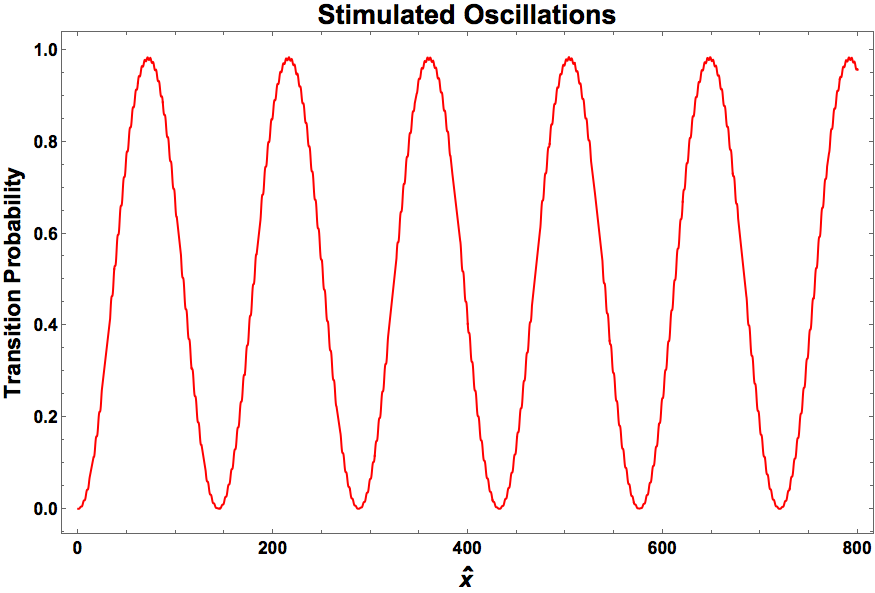
\includegraphics[width=0.85\textwidth]{assets/stimulated-oscillation-phenomenon.png}
%stimulated-neutrino-oscillations-kneller.png}
\caption*{Stimulated oscillation. $\delta \lambda(x) = A \sin (k x)$}
\end{figure}


}



%%% A text block that should be displayed later
\only<3->{
\begin{textblock*}{64mm}(32mm,0.4\textheight)

\begin{tcolorbox}
\centering
%\rotatebox{0}{
${\color{red}\delta\lambda(x)}$ is the problem here.
\begin{itemize}
    \item Varying background eigenenergy
    \item $\cdots$
\end{itemize}
%}
\vspace{1em}
\end{tcolorbox}

\end{textblock*}
}


\end{frame}







\section{Understanding Stimulated Oscillations}


\subsection{Hamiltonian, and Basis}

\begin{frame}{Understanding Stimulated Oscillations}

\begin{tcolorbox}[title=A Better Basis]

{\color{red}
Remove the position dependence of the diagonalized part of the Hamiltonian BY CHOOSING A NEW BASIS!
}

New basis where the wave function $(\psi_{p1},\psi_{p2})^T$ is related to the wave function in background matter basis through

\begin{equation*}
    \begin{pmatrix}
    \psi_1 \\
    \psi_2
    \end{pmatrix} = \begin{pmatrix}
     e^{-i \eta (x)} & 0 \\  0 & e^{i \eta (x)} 
    \end{pmatrix}\begin{pmatrix}
    \psi_{p1}\\
    \psi_{p2}
    \end{pmatrix},
\end{equation*}

where

\begin{equation*}
    \eta(x) - \eta(0) = - \frac{\omega_m}{2} x + \frac{\cos 2\theta_m}{2} \int_0^x \delta\lambda (\tau) d\tau.
\end{equation*}

\end{tcolorbox}

\begin{tcolorbox}[title=Transition Probability in Background Basis]

\begin{equation*}
    P_{1 \to 2} (x) = \left\lvert e^{i\eta} \psi_{p2} (x) \right \rvert^2 = \left\lvert \psi_{p2} (x)  \right\rvert^2 .
\end{equation*}

\end{tcolorbox}



\end{frame}



\begin{frame}{Understanding Stimulated Oscillations}



\only<1->{

% Background matter basis
\begin{itemize}
\item Hamiltonian in Background Matter Basis
    \begin{equation*}
    \mathbf {H_0} = \frac{1}{2}\left( - \omega_m + {\color{red}\delta \lambda(x)} \cos 2\theta_m \right) \boldsymbol{\sigma_3} - \frac{  {\color{red}\delta \lambda(x)}  }{2} \sin \theta_m \boldsymbol{\sigma_1}.
\end{equation*}

\item Hamiltonian in New Basis
\begin{equation*}
    \mathbf{H_p} = - \frac{ {\color{red}\delta \lambda(x)}  }{2} \sin 2\theta_m \begin{pmatrix} 0 & e^{2i\eta(x)} \\ e^{-2 i\eta(x) } & 0 \end{pmatrix} 
\end{equation*}    

\end{itemize}
}




\only<1>{
\begin{tcolorbox}[title=Rabi Oscillation]

Rabi oscillation Hamiltonian

\begin{equation*}
    \begin{pmatrix}
    E_1 & W \\
    W^* & E_2
    \end{pmatrix},
\end{equation*}

where $W$ is periodic, e.g., $e^{i k x}$.

\end{tcolorbox}

}

\only<2->{


\begin{tcolorbox}[title=Off-diagonal Term in Our System]

\begin{equation*}
e^{2i\eta (x)},
\end{equation*}

where
\begin{equation*}
\eta(x) - \eta(0) = - \frac{\omega_m}{2} x + \frac{\cos 2\theta_m}{2} \int_0^x {\color{red} \delta\lambda (\tau) }  d\tau.
\end{equation*}

\end{tcolorbox}

}



\end{frame}


\subsection{Single Frequency Matter Profile}

\begin{frame}{Single Frequency Matter Profile}


\begin{columns}[T]
\begin{column}{0.55\textwidth}

\begin{tcolorbox}[title=Matter Profile]

\begin{equation*}
    \lambda(x) = \lambda_0 + {\color{red} A \sin (k x)},
\end{equation*}

which leads to

\begin{equation*}
    {\color{violet}\eta(x)} = - \frac{\omega_m}{2}x {\color{blue}- \frac{\cos 2\theta_m}{2} \frac{A}{k} \cos (k x )}.
\end{equation*}

\end{tcolorbox}
\end{column}%

\begin{column}{0.45\textwidth}

\begin{tcolorbox}[title=Hamiltonian in New Basis]

\begin{equation*}
    -\frac{ {\color{red}\delta \lambda(x)}  }{2}\begin{pmatrix}
    0 & e^{2i {\color{violet}\eta(x)}  }\\
    e^{-2i {\color{violet}\eta(x)} } & 0
    \end{pmatrix}
\end{equation*}

\end{tcolorbox}

\end{column}

\end{columns}

The system can be (approximately) solved using Jacobi-Anger expansion

\begin{equation*}
e^{i z \cos ( k x)} = \sum_{n=-\infty}^\infty i^n J_n(z) e^{i n k x}.
\end{equation*}


\end{frame}




\begin{frame}{Single Frequency Matter Profile}

\only<1-1>{
\begin{tcolorbox}[title=Scaled Quantities]
Characteristic scale: $\omega_m$



\begin{itemize}
\item $\hat A = A/\omega_m$
    \item $\hat k = k/\omega_m$
    \item $\hat x = \omega x$
\end{itemize}
\end{tcolorbox}
}



\only<2-2>{
\begin{tcolorbox}[title=Rotation Wave Approximation]

The off-diagonal element of Hamiltonian

\begin{equation*}
\hat h= \sum_{n=-\infty}^{\infty} \frac{1}{2} \hat B_n e^{i  {\color{magenta} (n\hat k-1) } \hat x},
\end{equation*}

where $\hat B_n =  - (-i)^n  n \hat k \tan 2\theta_m  J_n ( \hat A \cos 2\theta_m / \hat k ) $.


${\color{magenta} (n \hat k-1) }$ $\to$ perturbation frequency in matter profile for each component.

\end{tcolorbox}


\begin{tcolorbox}[title=Which $n$ to Choose]
\centering
RWA: small ${\color{magenta} (n\hat k-1)}$ $\to$ important term

\centering
Find integer $n_0 = \mathrm{Round}\left[ 1/\hat k \right]$ that minimizes ${\color{magenta} n\hat k -1}$.

\end{tcolorbox}

}



\end{frame}




\begin{frame}{Single Frequency Matter Profile}


\begin{tcolorbox}[title=Transition Probability]

RWA $\to$ analytically solvable equation

\begin{equation*}
    P_{1\to 2} = \frac{ \lvert \Gamma/2 \rvert^2 }{ q ^2  } \sin^2 \left( \frac{q}{2} x \right)  ,
\end{equation*}

where

\begin{align*}
    q^2 &= \left\lvert  \Gamma/2 \right\rvert^2 + ( n_0 \hat k - 1 )^2,\qquad \text{frequency of oscillations} \\
    \Gamma &= \left\lvert \hat B_{n_0} \right\rvert, \qquad \text{width of resonance ($nk$ as parameter)} \\
    n_0 &= \mathrm{Round}\left[ 1/\hat k \right]
\end{align*}


\end{tcolorbox}


\end{frame}



\begin{frame}{Single Frequency Matter Profile}

\begin{figure}
    \centering
    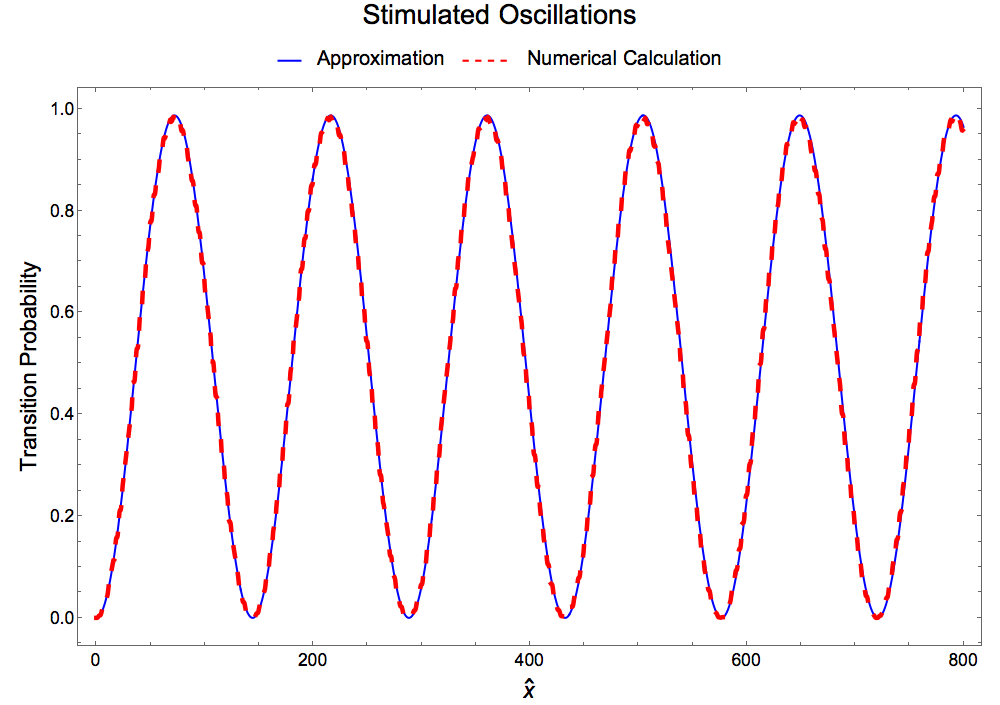
\includegraphics[width=0.9\textwidth]{assets/stimulated-oscillation-rwa-and-numerical.png}
    \caption*{RWA works. $\hat A=0.1$, $\hat k=0.995$, $\theta_m=\pi/6$}
\end{figure}

\end{frame}



\begin{frame}{Single Frequency Matter Profile}


\only<1-1>{

\begin{tcolorbox}[title=Why Does RWA Work?]

\begin{equation*}
    J_n(n \sech \alpha) \sim \frac{ e^{ - n(\alpha -\tanh\alpha )} }{ \sqrt{ 2\pi n \tanh \alpha } }, \quad \text{for large } n
\end{equation*}

% Hamiltonian off-diagonal element amplitude

% \begin{equation*}
%     \hat B_n \propto n J_n(n \sech \alpha) \sim \sqrt{n} \frac{ e^{ - n(\alpha -\tanh\alpha )} }{ \sqrt{ 2\pi  \tanh \alpha } }, \quad \text{for large } n
% \end{equation*}

% where $\sech\alpha = \hat A\cos 2\theta_m$.

$\Rightarrow$

\begin{equation*}
    \Gamma \propto \hat B_n \propto  \frac{ e^{ - n ( \alpha - \tanh \alpha )} }{\sqrt{2\pi n \tanh \alpha} } 
\end{equation*}

Small perturbation $\Rightarrow$ Small $\hat A$ $\Rightarrow$ Large $\alpha$ $\Rightarrow$ Drops fast at large $n$.


\end{tcolorbox}
}

\end{frame}



% \begin{frame}{Single Frequency Matter Profile}


% \begin{tcolorbox}[title=PLACEHOLDER]
% \color{red}
% NEED A GRAPH TO EXPLAIN WHY FOR A SPECIFIC n WE ONLY TAKE THE ONE THAT IS MOST CLOSE TO RESONANCE!!!

% \end{tcolorbox}



% \end{frame}




\begin{frame}{Single Frequency Matter Profile}




% \only<1-1>{

% \begin{figure}
% \centering
% 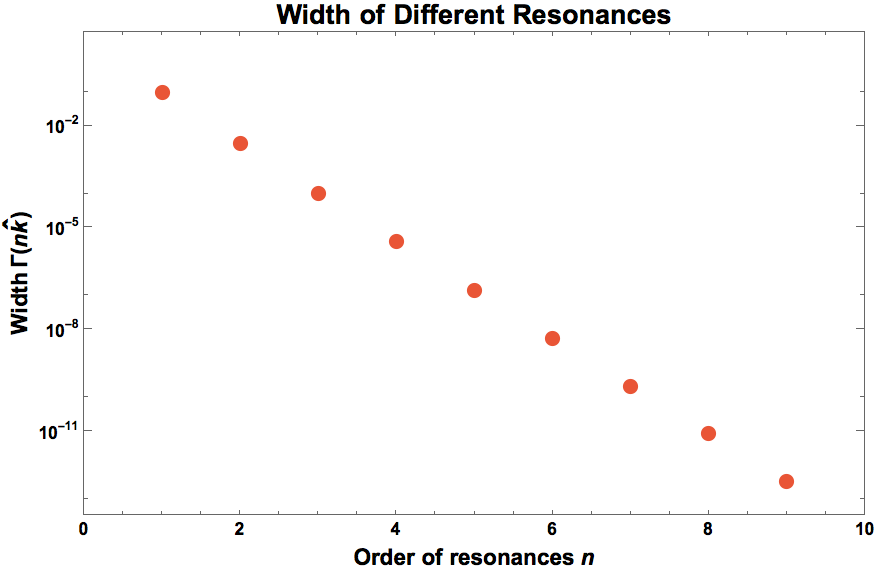
\includegraphics[width=0.9\textwidth]{assets/stimulated-single-frequency-width-nk-orders.png}
% \caption*{Width of the resonances for $A=0.1$, $\theta_m = \pi/5$. Each width is a parameter of $n \hat k$.}
% \end{figure}

% }


%\only<2-2>{

\begin{figure}
\centering
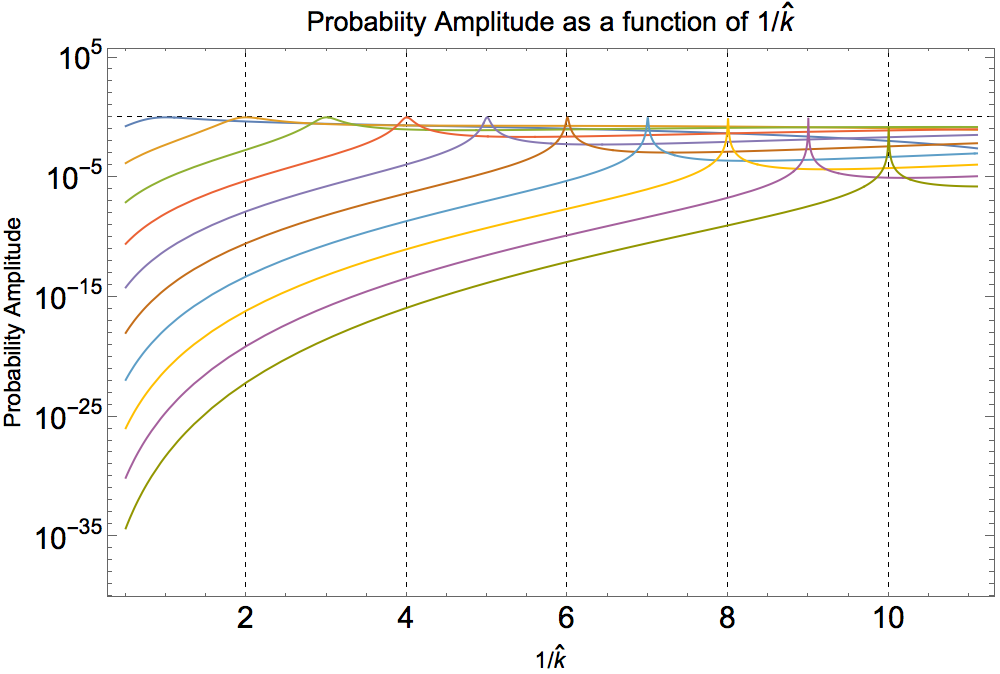
\includegraphics[width=0.9\textwidth]{assets/stimulated-single-frequency-resonances-k-orders.png}
\caption*{Transition probability amplitude as a function of $1/\hat k$  (the phase is $(n - 1/\hat k)$). The colors represent different orders of $n_0$.}
\end{figure}

%}


\end{frame}


\subsection{Two-frequency Matter Profile}


\begin{frame}{Two-frequency Matter Profile}


\only<1-1>{
\begin{tcolorbox}[title=Matter Profile]

\begin{equation*}
    \lambda(x) = \lambda_0 + \color{red}\delta\lambda(x),\quad     \color{red}\delta \lambda(x) = A_1 \sin (k_1 x) +  A_2 \sin (k_2 x).
\end{equation*}
\end{tcolorbox}
}

\only<2->{
\begin{tcolorbox}[title=Hamiltonian Off-diagonal Element]

Apply Jacobi-Anger expansion,

\begin{equation*}
\hat h  = \sum_{n_1=-\infty}^\infty \sum_{n_2=-\infty}^{\infty}  \frac{1}{2} \hat B_{n_1,n_2}(\hat k_1,\hat k_2)
 e^{i(n_1 \hat k_1 + n_2 \hat k_2 - 1)\hat x},
\end{equation*}

where

\begin{align*}
&\hat B_{n_1,n_2}( \hat k_1,\hat k_2)\\
= & -(-i)^{n_1+n_2} ( n_1 \hat k_1 + n_2 \hat k_2 ) J_{n_1}\left( \frac{\hat A_1\cos 2\theta_m}{\hat k_1} \right) J_{n_2}\left( \frac{\hat A_2\cos 2\theta_m}{\hat k_2} \right) 
\end{align*}


\end{tcolorbox}
}


\only<2->{
\begin{tcolorbox}
\centering
\color{red}Which terms are important?
\end{tcolorbox}

}

\only<2->{

\begin{textblock*}{64mm}(68mm,0.01\textheight)

\small
\begin{equation*}
\hat h=\sum_{n=-\infty}^{\infty} \frac{1}{2} \hat B_n e^{i  {\color{magenta} (n\hat k-1) } \hat x},
\end{equation*}
\normalsize

\end{textblock*}


}




\end{frame}



\begin{frame}{Two-frequency Matter Profile}

\only<1-1>{
\begin{tcolorbox}[title=Resonance Lines]

There are still resonances, i.e., (almost) zero phases, on lines

\begin{equation*}
    n_{1,0} \hat k_1 + n_{2,0} \hat k_2 -1 =0
\end{equation*}

in $\{\hat k_1,\hat k_2\}$ plane. 
{\centering
$\Rightarrow$
}
Resonance width for each point on resonance lines.

\end{tcolorbox}
}

\only<2-2>{

\begin{figure}
    \centering
    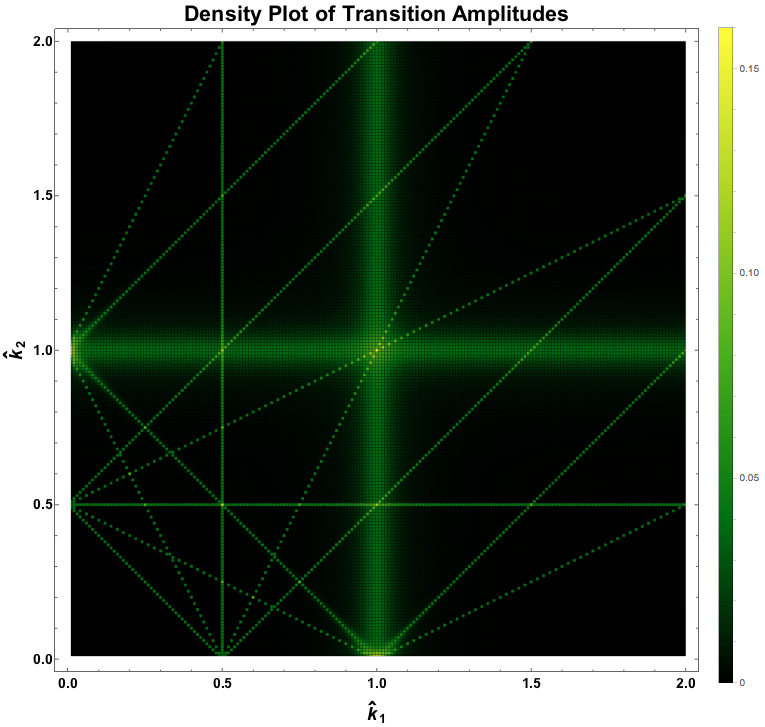
\includegraphics[width=0.7\textwidth]{assets/density-plot-of-transition-amplitudes-demonstration.png}
    \caption*{Density plot of transition amplitudes calculated using only one term out of the whole summation in Hamiltonian. $n_1,n_2\in [-2, 2]$}
\end{figure}

\begin{textblock*}{64mm}(70mm,0.01\textheight)
\tiny
\begin{equation*}
\hat h  = \sum_{n_1} \sum_{n_2}  \frac{1}{2} \hat B_{n_1,n_2}(\hat k_1, \hat k_2)
 e^{i(n_1 \hat k_1 + n_2 \hat k_2 - 1)\hat x},
\end{equation*}
\normalsize
\end{textblock*}

}


\only<3->{
\begin{figure}
    \centering
    \includegraphics[width=0.75\textwidth]{assets/stimulated-2-freq-width-diagram.png}
    \caption*{Resonance line, distance to resonance, and width}
\end{figure}
}



\end{frame}



\begin{frame}{Two-frequency Matter Profile}


\begin{tcolorbox}[title=Width]

\begin{equation*}
    \Gamma_2 = \frac{\hat B_{n_1,n_2}(\hat k_{1,\mathrm{intercept}}, \hat k_{2,\mathrm{intercept}})}{\sqrt{n_1^2 + n_2^2}}.
\end{equation*}

\end{tcolorbox}


\begin{tcolorbox}[title=Distance to Resonance Line]

\begin{equation*}
d = \frac{\lvert n_1 \hat k_{10} + n_2 \hat k_{20} - 1 \rvert}{\sqrt{n_1^2 + n_2^2} }.
\end{equation*}

\end{tcolorbox}


\begin{tcolorbox}[title=Distance to Resonance Width Ratio]

\begin{equation*}
Q_2 = \frac{d}{\Gamma_2}.    
\end{equation*}


\end{tcolorbox}

\end{frame}


\begin{frame}{Two-frequency Matter Profile}



\only<1-1>{
\begin{figure}
    \centering
    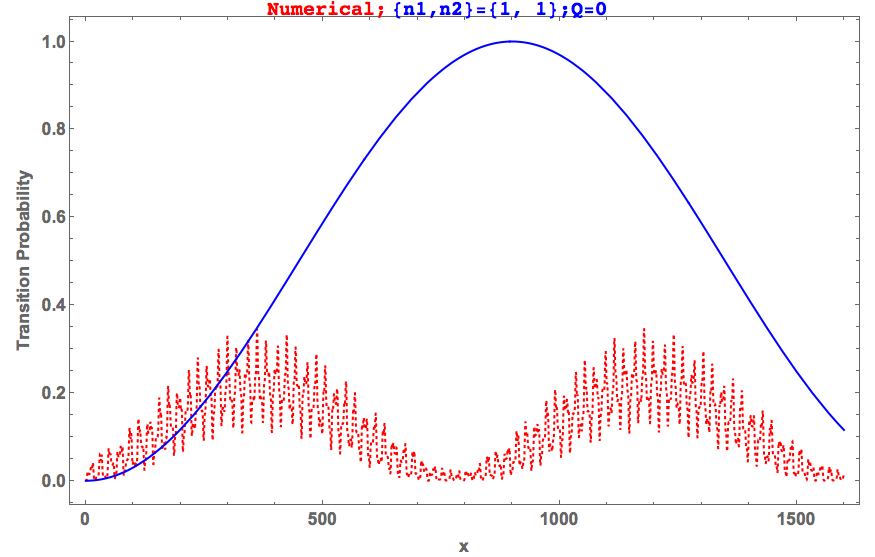
\includegraphics[width=0.9\textwidth]{assets/q-ordering-1.png}
    \caption*{}
\end{figure}
}


\only<2-2>{
\begin{figure}
    \centering
    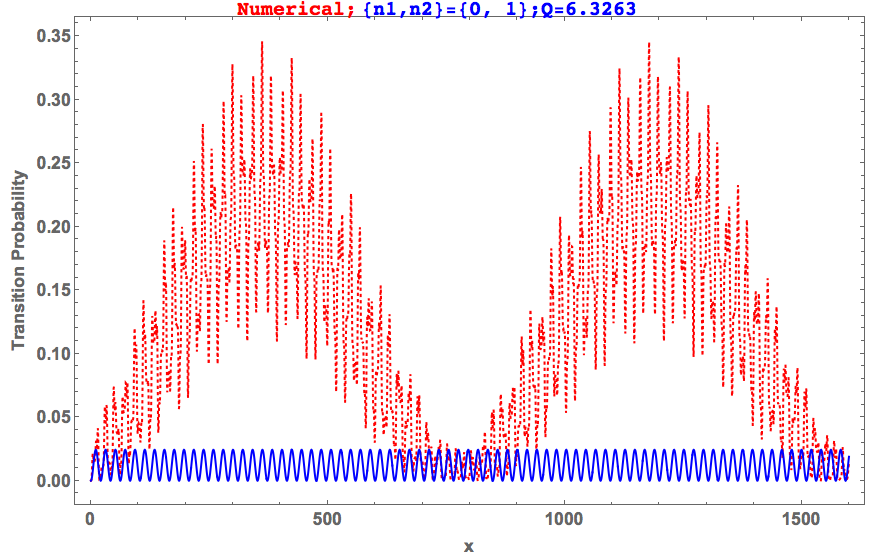
\includegraphics[width=0.9\textwidth]{assets/q-ordering-2.png}
    \caption*{}
\end{figure}
}


\only<3-3>{
\begin{figure}
    \centering
    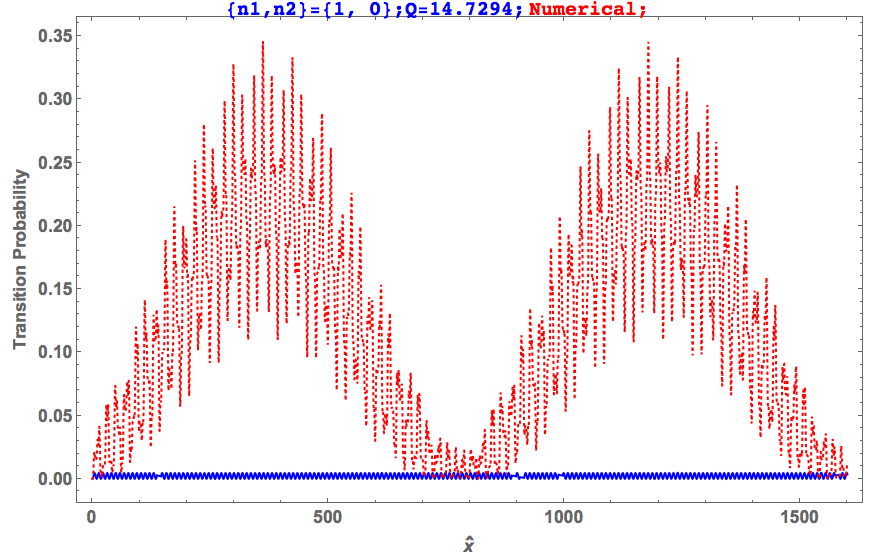
\includegraphics[width=0.9\textwidth]{assets/q-ordering-3.png}
    \caption*{}
\end{figure}
}

\only<4-4>{
\begin{figure}
    \centering
    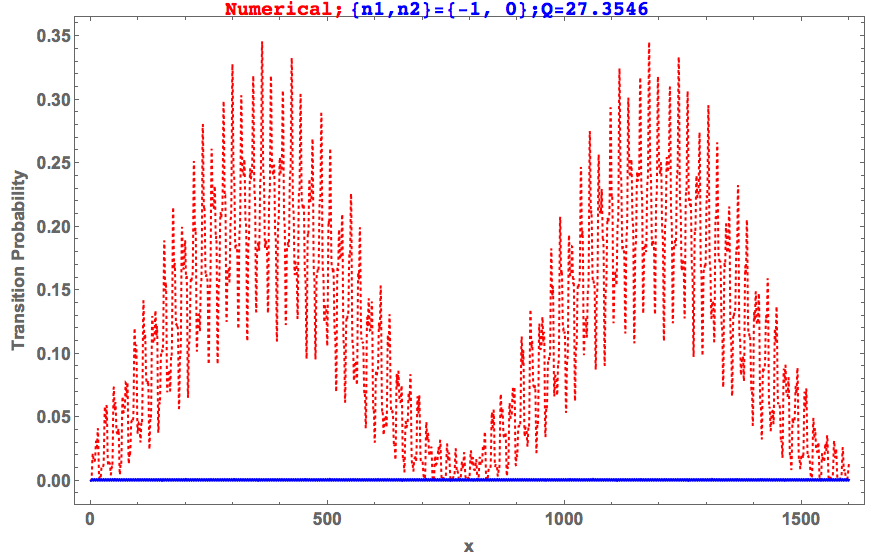
\includegraphics[width=0.9\textwidth]{assets/q-ordering-4.png}
    \caption*{}
\end{figure}
}

\only<5-5>{
\begin{figure}
    \centering
    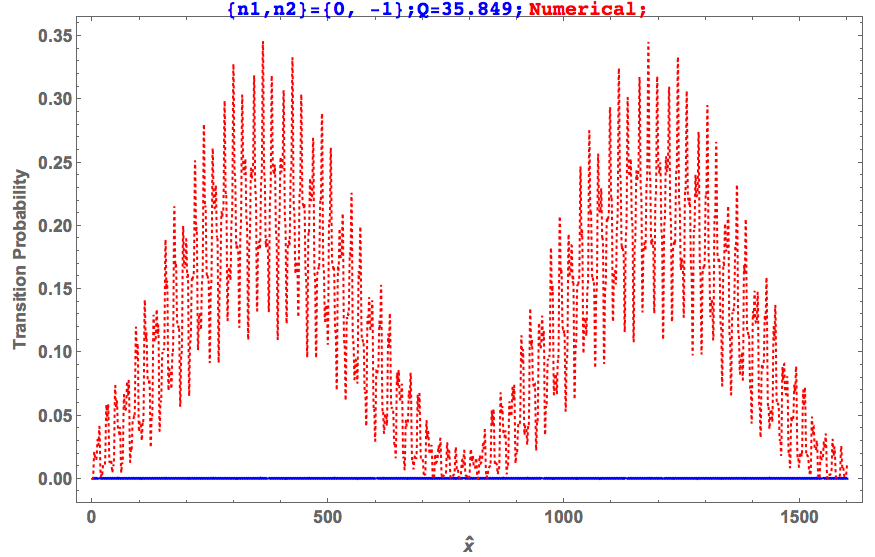
\includegraphics[width=0.9\textwidth]{assets/q-ordering-5.png}
    \caption*{}
\end{figure}
}

\only<6-6>{
\begin{figure}
    \centering
    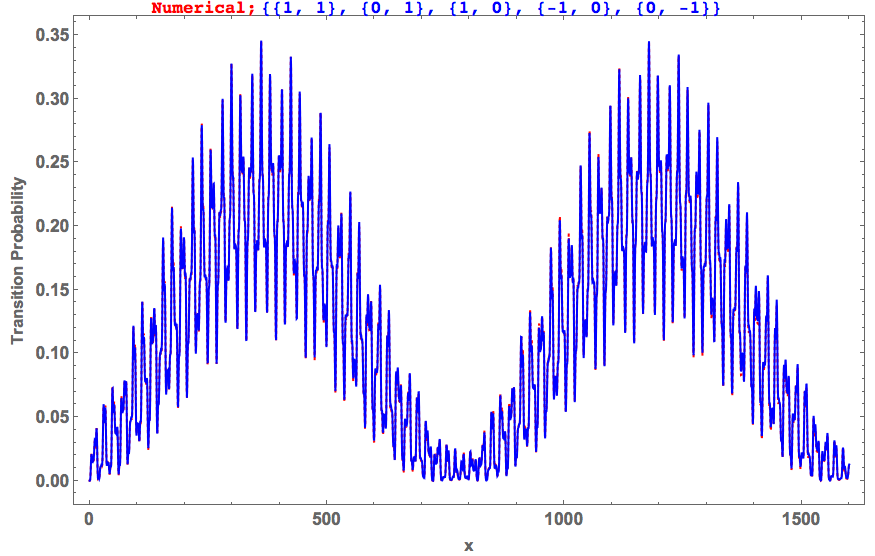
\includegraphics[width=0.9\textwidth]{assets/2-freq-numerical-and-first-5-rwa.png}
    \caption*{}
\end{figure}
}

\end{frame}




%%%%%%%%%%%%%%%%%%%%%%%%%%%%%%%%%%%%%%%%%%%%%%%%%
%%%%%%% Summary & Outlook/Future Work %%%%%%%%%%%%%%

% You should see now what I am trying to do here.
% In reality, a matter profile can be decomposed into many Fourier modes. If we can find a way to determine which terms are important, it would be very useful for more complicated calculations such as the combination of COLLECTIVE neutrino oscillations and matter effect.
% Rather easy to numerically solve such systems. However, it is also good to learn the physics behind numerical calculation. Look into the most important term.

\section{Summary \& Future Work}

\begin{frame}{Summary \& Future Work}



\begin{itemize}\color{ao}
\item 
Matter interaction depends on matter profile
\item
Single frequency periodic matter profile can be approximated using lowest order of RWA.
\item
Two frequency periodic matter profile can be calculated using some lowest orders of RWA.

\end{itemize}



\begin{itemize}\color{red}
 \item 
 Multi-frequency matter profile
 
\end{itemize}




\end{frame}



\begin{frame}{Acknowledgement}



\end{frame}







\appendix

\begin{frame}[fragile]{Backup slides}
  Sometimes, it is useful to add slides at the end of your presentation to
  refer to during audience questions.

  The best way to do this is to include the \verb|appendixnumberbeamer|
  package in your preamble and call \verb|\appendix| before your backup slides.

  \themename will automatically turn off slide numbering and progress bars for
  slides in the appendix.
\end{frame}

\begin{frame}[allowframebreaks]{References}

  \bibliography{ref}
  \bibliographystyle{abbrv}

\end{frame}

\end{document}
